
%% bare_conf.tex
%% V1.3
%% 2007/01/11
%% by Michael Shell
%% See:
%% http://www.michaelshell.org/
%% for current contact information.
%%
%% This is a skeleton file demonstrating the use of IEEEtran.cls
%% (requires IEEEtran.cls version 1.7 or later) with an IEEE conference paper.
%%
%% Support sites:
%% http://www.michaelshell.org/tex/ieeetran/
%% http://www.ctan.org/tex-archive/macros/latex/contrib/IEEEtran/
%% and
%% http://www.ieee.org/

%%*************************************************************************
%% Legal Notice:
%% This code is offered as-is without any warranty either expressed or
%% implied; without even the implied warranty of MERCHANTABILITY or
%% FITNESS FOR A PARTICULAR PURPOSE! 
%% User assumes all risk.
%% In no event shall IEEE or any contributor to this code be liable for
%% any damages or losses, including, but not limited to, incidental,
%% consequential, or any other damages, resulting from the use or misuse
%% of any information contained here.
%%
%% All comments are the opinions of their respective authors and are not
%% necessarily endorsed by the IEEE.
%%
%% This work is distributed under the LaTeX Project Public License (LPPL)
%% ( http://www.latex-project.org/ ) version 1.3, and may be freely used,
%% distributed and modified. A copy of the LPPL, version 1.3, is included
%% in the base LaTeX documentation of all distributions of LaTeX released
%% 2003/12/01 or later.
%% Retain all contribution notices and credits.
%% ** Modified files should be clearly indicated as such, including  **
%% ** renaming them and changing author support contact information. **
%%
%% File list of work: IEEEtran.cls, IEEEtran_HOWTO.pdf, bare_adv.tex,
%%                    bare_conf.tex, bare_jrnl.tex, bare_jrnl_compsoc.tex
%%*************************************************************************

% *** Authors should verify (and, if needed, correct) their LaTeX system  ***
% *** with the testflow diagnostic prior to trusting their LaTeX platform ***
% *** with production work. IEEE's font choices can trigger bugs that do  ***
% *** not appear when using other class files.                            ***
% The testflow support page is at:
% http://www.michaelshell.org/tex/testflow/



% Note that the a4paper option is mainly intended so that authors in
% countries using A4 can easily print to A4 and see how their papers will
% look in print - the typesetting of the document will not typically be
% affected with changes in paper size (but the bottom and side margins will).
% Use the testflow package mentioned above to verify correct handling of
% both paper sizes by the user's LaTeX system.
%
% Also note that the "draftcls" or "draftclsnofoot", not "draft", option
% should be used if it is desired that the figures are to be displayed in
% draft mode.
%
\documentclass[conference,onecolumn]{IEEEtran}
% Add the compsoc option for Computer Society conferences.
%
% If IEEEtran.cls has not been installed into the LaTeX system files,
% manually specify the path to it like:
% \documentclass[conference]{../sty/IEEEtran}

\usepackage[numbers]{natbib}
\usepackage{amsmath}
\usepackage{hyperref}
\usepackage{amsfonts}
\usepackage{booktabs}
\usepackage{xspace}
\usepackage{graphicx}

\usepackage{subfigure}
\newcommand{\algorithmCTxt}{Ordered Confidence Bound\xspace}
\newcommand{\algorithmCFname}{OrderedConfidenceBound}
\newcommand{\algorithmDTxt}{Prior Confidence Bound\xspace}
\newcommand{\algorithmDFname}{PriorConfidenceBound}

%\newcommand{\jgonote}[1]{\textcolor{blue}{\textbf{JGO: #1}}}


% correct bad hyphenation here
\hyphenation{op-tical net-works semi-conduc-tor}


\begin{document}
%
% paper title
% can use linebreaks \\ within to get better formatting as desired
\title{Learning to Pick Up Objects Through Active Exploration}


% author names and affiliations
% use a multiple column layout for up to three different
% affiliations
\author{\IEEEauthorblockN{John Oberlin and Stefanie Tellex}
\IEEEauthorblockA{Computer Science Department, Brown University}}


% conference papers do not typically use \thanks and this command
% is locked out in conference mode. If really needed, such as for
% the acknowledgment of grants, issue a \IEEEoverridecommandlockouts
% after \documentclass

% for over three affiliations, or if they all won't fit within the width
% of the page, use this alternative format:
% 
%\author{\IEEEauthorblockN{Michael Shell\IEEEauthorrefmark{1},
%Homer Simpson\IEEEauthorrefmark{2},
%James Kirk\IEEEauthorrefmark{3}, 
%Montgomery Scott\IEEEauthorrefmark{3} and
%Eldon Tyrell\IEEEauthorrefmark{4}}
%\IEEEauthorblockA{\IEEEauthorrefmark{1}School of Electrical and Computer Engineering\\
%Georgia Institute of Technology,
%Atlanta, Georgia 30332--0250\\ Email: see http://www.michaelshell.org/contact.html}
%\IEEEauthorblockA{\IEEEauthorrefmark{2}Twentieth Century Fox, Springfield, USA\\
%Email: homer@thesimpsons.com}
%\IEEEauthorblockA{\IEEEauthorrefmark{3}Starfleet Academy, San Francisco, California 96678-2391\\
%Telephone: (800) 555--1212, Fax: (888) 555--1212}
%\IEEEauthorblockA{\IEEEauthorrefmark{4}Tyrell Inc., 123 Replicant Street, Los Angeles, California 90210--4321}}




% use for special paper notices
%\IEEEspecialpapernotice{(Invited Paper)}




% make the title area
\maketitle


% IEEEtran.cls defaults to using nonbold math in the Abstract.
% This preserves the distinction between vectors and scalars. However,
% if the conference you are submitting to favors bold math in the abstract,
% then you can use LaTeX's standard command \boldmath at the very start
% of the abstract to achieve this. Many IEEE journals/conferences frown on
% math in the abstract anyway.

% no keywords




% For peer review papers, you can put extra information on the cover
% page as needed:
% \ifCLASSOPTIONpeerreview
% \begin{center} \bfseries EDICS Category: 3-BBND \end{center}
% \fi
%
% For peerreview papers, this IEEEtran command inserts a page break and
% creates the second title. It will be ignored for other modes.
\IEEEpeerreviewmaketitle


Robots need to perceive and manipulate objects in its environment, yet
robust object manipulation remains a challenging problem.  Many
aspects of a perception and manipulation system need to be customized
for a particular object and environment, such as where to grasp an
object, what algorithm to use for segmentation, and what height to
visually servo above an object on the table.  To address these
limitations, we propose an approach for enabling a robot to learn
about objects through active exploration and adapt its grasping model
accordingly.  We frame the problem of model adaptation as a bandit
problem, specifically the identification of the best of the arms of an
N-armed bandit, ~\citep{thompson33} where the robot aims to minimize
simple regret after a finite exploration period~\citep{bubeck09}.  Our
robot can obtain a high-quality reward signal (although sometimes at a
higher cost in time and sensing) by actively collecting additional
information from the environment, and use this reward signal to
adaptively identify grasp points that are likely to succeed.  This
paper provides an overview of our previous work~\citep{oberlin15}
using this approach to actively infer grasp points and adds a
description of our efforts learning the height to servo to an object.

We use our robot's eye-in-hand camera to visually servo to an object
and identify it; however, objects have different sizes. Some objects
are large, and need to be observed from far away so that the entire
object fits in frame, but not too far because the precision of the
alignment process falls with the distance from the object as pixels in
the image span larger physical distances.  On the other hand, small
objects should be observed more closely to obtain a higher-resolution
image and finer-grained pose estimation, but not too closely because
distortions in the transformations between camera and physical
coordinates become more dramatic when the object is nearer the lens.

Our previous work~\citep{oberlin15} presented a new algorithm,
\algorithmDTxt, based on Hoeffding races~\citep{maron93}. In our
approach, the robot pulls arms in an order determined by a prior,
which allows it to try the most promising arms first. It can then
autonomously decide when to stop exploring by bounding the confidence
in the result.  Figure~\ref{fig:height} shows the robot's performance
on two differently sized objects; after training it servos at a higher
height for the epipen, which is larger, and a lower height for the
egg, improving the success rate.  The contribution of this short paper
is to apply our algorithm to learn what height to observe an object.

Formally, the agent is given an N-armed bandit, where each arm pays
out $1$ with probability $\mu_i$ and $0$ otherwise.  The agent's goal
is to identify a good arm (with payout $>= k$) with probability $c$
(e.g., 95\% confidence that this arm is good) as quickly as possible.
As soon as it has done this, it should terminate.  The agent is also
given a prior $\pi$ on the arms so that it may make informed decisions
about which arm to explore.



%% We use slower, more accurate sensing approaches
%% to provide supervision for faster, simpler methods that excel with
%% large amounts of training data.  For example, to perform grasping we
%% use an analytic model to select grasp points, but depending on the
%% object, the best grasp according to the analytic model may not be
%% optimal; the robot can learn better grasps for that object using the
%% analytic model as a prior and actively collecting data for that
%% object.

%%  a view-based model for closed-loop visual picking.  View-based
%% methods for instance detection have many advantages over methods using
%% 3D models, because they directly capture the visual appearance of the
%% object, and are relatively simple and efficient to implement because
%% they operate on low-level features~\citep{hsiao13}.  However these
%% systems require large amounts of training data for robust performance,
%% for example more than 2000 images which must be manually collected and
%% annotated with bounding boxes for the state of the art LINE2D
%% method~\citep{hinterstoisser12}.  Moreover, for manipulation,
%% view-based methods do not propose potential grasps, and autonomous
%% methods for recognizing visual grasps are prone to error. 

%% To address these issues, we present an approach for enabling a robot
%% to train its own view-based model to recognize and manipulate the
%% specific objects it will need to use during collaborations with
%% humans.  Using our algorithm, the robot detects candidate objects for
%% training using a depth sensor, then actively collects view-based
%% visual templates to perform robust instance-based object detection,
%% pose estimation and closed-loop grasping using visual servoing.
%% Because our camera can move with seven degrees of freedom, the robot
%% can collect large quantities of data leading to simple visual models
%% that perform with high accuracy even under occlusion.  Our approach is
%% enabled by three innovations: our end-to-end algorithm for collecting
%% view-based training data with supervision obtained from a
%% higher-reliability depth sensor, which is supported by a simple and
%% robust method for determining candidate grasps using a depth sensor
%% mounted on a seven-degree-of-freedom arm, along with an approach for
%% autonomously and reliably finding object bounding boxes once the
%% object is on a background such as a floor or table.


Our approach iteratively chooses the arm with the highest observed (or
prior) success rate but whose probability of being below $k$ is less
than $c$. It then tries that arm, records the results, and checks to
see if its probability of success is above $k$ or within $[k-\epsilon,
  k+\epsilon]$ with probability $c$ (in which case it terminates). (If
the latter condition is not included, an arm with success probability
equal to $k$ will continue to be pulled indefinitely.)  We need to
estimate the probability that the true payout probability, $\mu$, is
greater than the threshold, $c$, given the observed number of
successes and failures:
\begin{align}
\Pr(\mu_i > c|  S, F)
\end{align}
\noindent We can compute this probability using the law of total
probability: $\Pr(\mu_i > c| S, F) = 1 - \int_0^k \Pr(\mu_i=\mu | S,
F) d\mu$, assuming a beta distribution on $\mu$: $\int_k^1 \mu^S (1-
\mu) ^F d\mu$.  This integral is the CDF of the beta distribution, and
is called the regularized incomplete beta function~\citep{olver10}.

In our previous work, the space of possible arms was defined by
different grasp points on the object.  In this paper, we optimize an
additional parameter from experience: the height above the table.
Each arm is the height above the table, and reward is defined by the
ability to servo twice and end up at the same x,y location, when the
object hasn't moved.  If the robot can servo consistently to the same
location on the object, this signal is an indication that it is a good
height.

\section*{Evaluation}


\begin{figure}
\parbox{0.5\linewidth}{
\subfigure[The robot learns to servo for the epipen at a higher height, so the entire object fits in frame; it servos the egg at a lower height to obtain higher positional accuracy.\label{fig:height}]{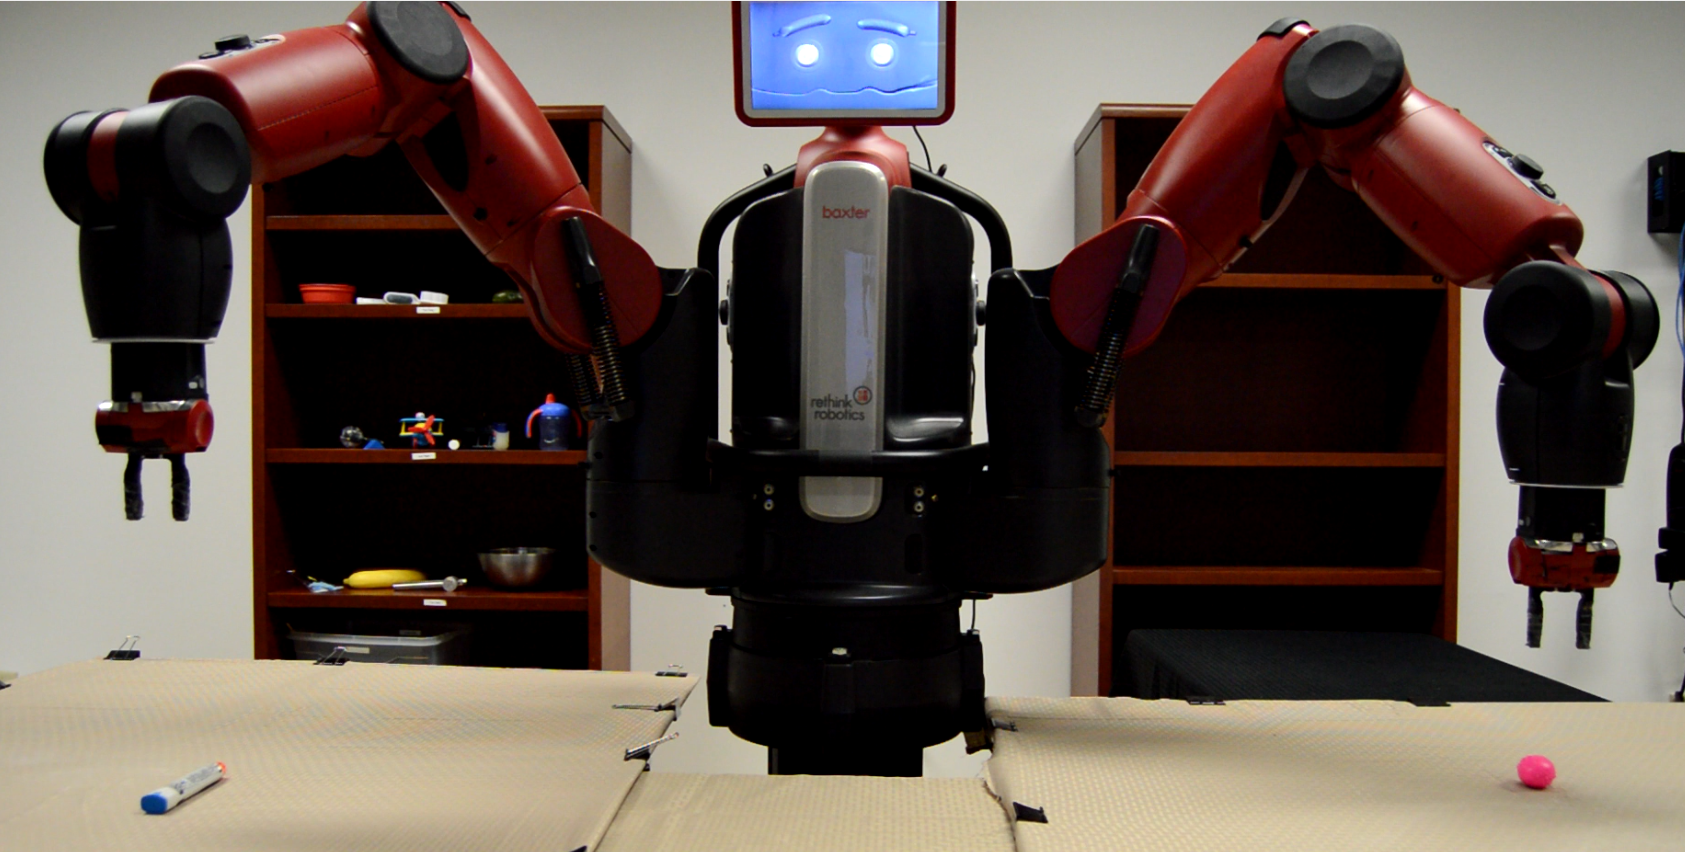
\includegraphics[width=1\linewidth]{figures/epipen_egg.jpg}}

%\subfigure[Before learning, the robot grasps the ruler near the end and drops it; after learning, it grasps it near the middle.\label{fig:ruler}]{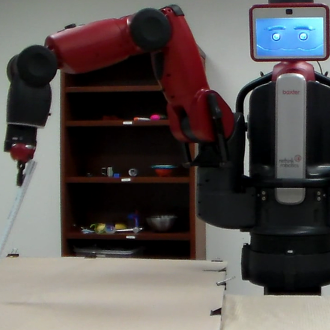
\includegraphics[width=0.5\linewidth]{figures/dropping_ruler.png}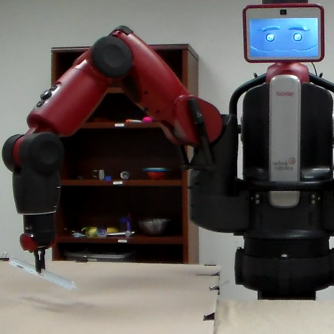
\includegraphics[width=0.5\linewidth]{figures/holding_ruler.png}}

\subfigure[Objects in our evaluation, which improves grasping performance from 55\% (before learning) to 75\% (after learning).\label{fig:object_glory_shot}]{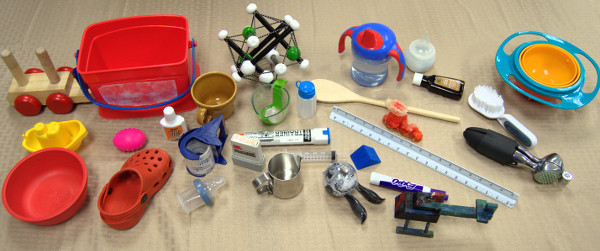
\includegraphics[width=1\linewidth]{figures/object_glory_shot.jpg}}
}%
\subfigure[Quantitative results.\label{table:robot_results}]{\parbox{0.5\linewidth}{
\tiny \centering
\begin{tabular}{cccc}
\toprule
		    & Prior         &  Training     & Marginal\\
\midrule
\multicolumn{4}{c}{$\Delta = 0; training = 3$} \\
\midrule
Garlic Press        & 0/10          &  8/50        &  2/10 \\
Gyro Bowl    	    & 0/10          &  5/15        &  3/10 \\
Helicopter    	    & 2/10          &  8/39        &  3/10 \\
Big Syringe    	    & 1/10          &  13/50       &  4/10 \\
Clear Pitcher       & 4/10          &  3/4         &  4/10 \\
Sippy Cup    	    & 0/10          &  6/50        &  4/10 \\
Red Bucket    	    & 5/10          &  3/3         &  5/10 \\
Dragon    	    & 8/10          &  5/6         &  7/10 \\
Ruler    	    & 6/10          &  5/12        &  7/10 \\
Triangle Block      & 0/10          &  3/13        &  7/10 \\
Bottle Top    	    & 0/10          &  5/17        &  7/10 \\
Wooden Spoon        & 7/10          &  3/3         &  7/10 \\
Icosahedron    	    & 7/10          &  7/21        &  8/10 \\
Blue Salt Shaker    & 6/10          &  5/10        &  8/10 \\
Epipen    	    & 8/10          &  4/5         &  8/10 \\
Wooden Train        & 4/10          &  11/24       &  8/10 \\
Stamp    	    & 8/10          &  3/3         &  8/10 \\
Toy Egg    	    & 8/10          &  4/5         &  9/10 \\
Yellow Boat    	    & 9/10          &  5/6         &  9/10 \\
Vanilla	   	    & 5/10          &  4/5         &  9/10 \\
Round Salt Shaker   & 1/10          &  4/16        &  9/10 \\
Packing Tape        & 9/10          &  3/3         &  9/10 \\
Purple Marker       & 9/10          &  3/3         &  9/10 \\
Whiteout    	    & 10/10         &  3/3         &  10/10\\
Syringe    	    & 9/10          &  6/9         &  10/10\\
Brush    	    & 10/10         &  3/3         &  10/10\\
Red Bowl    	    & 10/10         &  3/3         &  10/10\\
Shoe    	    & 10/10         &  3/3         &  10/10\\
Metal Pitcher       & 6/10          &  7/12        &  10/10\\
Mug    		    & 3/10          &  3/4         &  10/10\\
\midrule
Total		    & 165/300       &  148/400     & 224/300\\
Rate		    & 0.55          &  0.37        & 0.75\\
\bottomrule
\end{tabular}
~\\~
~\\~
}}
\caption{Results from our evaluation. \label{fig:evaluation}}
\end{figure}

We implemented our approach on the Baxter robot.  The robot acquired
visual and RGB-D models for 30 objects using our autonomous learning
system.  The objects used in our evaluation appear in
Figure~\ref{fig:object_glory_shot}.  After acquiring visual and IR
models for the object at different poses of the arm and camera, the
robot performed the bandit-based adaptation step.  After the robot
detects an initially successful grasp, it shakes the object vigorously
to ensure that it would not fall out during transport. After releasing
the object and moving away, the robot checks to make sure the object
is not stuck in its gripper. If the object falls out during shaking or
does not release properly, the grasp is recorded as a failure. If the
object is stuck, the robot pauses and requests assistance before
proceeding.

Most objects have more than one pose in which they can stand upright
on the table. If the robot knocks over an object, the model taken in
the reference pose is no longer meaningful. Thus, during training, we
monitored the object and returned it to the reference pose whenever
the robot knocked it over. In the future, we aim to incorporate
multiple components in the models which will allow the robot to cope
with objects whose pose can change during training.

Our evaluation demonstrates that our adaptation step improves the
overall pick success rate from 55\% to 75\% on our test set of 30
household objects, shown in Figure~\ref{fig:object_glory_shot}, after
doing pick and height training.  Height servoing allows the robot to
adjust to different heights as shown in Figure~\ref{fig:height}.
Video showing our approach and evaluation can be seen at
\url{https://www.youtube.com/watch?v=xfH0B3g782Y}.

\section*{Conclusion}

Our robotic system gathers feedback from the environment, which it
uses to learn models to detect, localize, and manipulate previously
unseen objects.  This paper demonstrates that our approach can learn
to servo at different heights for different objects.  In the future,
we plan to explore learning parameters for a wider variety of tasks.
For instance, we use color gradients for localization,
but some objects would work better with other quantities. One could
learn the appropriate map to use when localizing each object, or even
further, the map might also depend upon the robot's current
environment.
%\jgonote{this reads really nicely}

Instance-based approaches mean that the robot must acquire data about
a specific object before manipulating it; however by adapting itself
to the object it can obtain higher accuracy.  We aim to aggregate data
collected via our instance-based system to create a new data set of
images, RGB-D, and grasp success rates at various poses to provide
supervision for general-purpose category models for grasping.  Our
long term vision is a system that can infer high quality grasps for
any object, but adaptively recover if the initial grasp attempt is
unsuccessful, leading overall to robust and accurate pick-and-place.



% trigger a \newpage just before the given reference
% number - used to balance the columns on the last page
% adjust value as needed - may need to be readjusted if
% the document is modified later
%\IEEEtriggeratref{8}
% The "triggered" command can be changed if desired:
%\IEEEtriggercmd{\enlargethispage{-5in}}

% references section

% can use a bibliography generated by BibTeX as a .bbl file
% BibTeX documentation can be easily obtained at:
% http://www.ctan.org/tex-archive/biblio/bibtex/contrib/doc/
% The IEEEtran BibTeX style support page is at:
% http://www.michaelshell.org/tex/ieeetran/bibtex/
%\bibliographystyle{IEEEtran}
% argument is your BibTeX string definitions and bibliography database(s)
%\bibliography{IEEEabrv,../bib/paper}
%
% <OR> manually copy in the resultant .bbl file
% set second argument of \begin to the number of references
% (used to reserve space for the reference number labels box)
{\tiny
\bibliographystyle{plainnat}
\bibliography{main}
}



% that's all folks
\end{document}


